%
%                       This is a basic LaTeX Template
%                       for the Informatics Research Review

\documentclass[a4paper,11pt]{article}
% Add local fullpage and head macros
\usepackage{head,fullpage}
% Add graphicx package with pdf flag (must use pdflatex)
\usepackage[pdftex]{graphicx}
% Better support for URLs
\usepackage{url}
% Date formating
\usepackage{datetime}
% For Gantt chart
\usepackage{pgfgantt}
\usepackage{xcolor}
\usepackage[utf8]{inputenc}

\newdateformat{monthyeardate}{%
  \monthname[\THEMONTH] \THEYEAR}

\parindent=0pt          %  Switch off indent of paragraphs
\parskip=5pt            %  Put 5pt between each paragraph
\Urlmuskip=0mu plus 1mu %  Better line breaks for URLs


%                       This section generates a title page
%                       Edit only the following three lines
%                       providing your exam number,
%                       the general field of study you are considering
%                       for your review, and name of IRR tutor

\newcommand{\examnumber}{B131025}
\newcommand{\field}{Emergen of Numeral System in \\ Multi-agent Autonomous Communication}
\newcommand{\tutor}{Prof. Stuart Anderson}
\newcommand{\supervisor}{Dr. Ivan Titov}

% added by Shawn
\usepackage{url}
\usepackage{breakcites}

\begin{document}
\begin{minipage}[b]{110mm}
        {\Huge\bf School of Informatics
        \vspace*{17mm}}
\end{minipage}
\hfill
\begin{minipage}[t]{40mm}
        \makebox[40mm]{
        
\includegraphics[width=40mm]{crest.png}}
\end{minipage}
\par\noindent
    % Centre Title, and name
\vspace*{2cm}
\begin{center}
        \Large\bf Informatics Project Proposal \\
        \Large\bf \field
\end{center}
\vspace*{1.5cm}
\begin{center}
        \bf \examnumber\\
        \monthyeardate\today
\end{center}
\vspace*{5mm}

%
%                       Insert your abstract HERE
%
\begin{abstract}
This project aims to develop a new framework for simulating the emergence of numeral system based on multi-agent autonomous communication system following deep reinforcement learning methodology. Under this new framework, we do not need to assign any linguistic knowledge to computer models any more. Instead, we can facilitate computational agents to invent their numeral system all from scratch. Thus, this project can help us to evaluate not only the assumptions about the emergence of numeral systems in natural language but the importance of certain factors in this procedure. From the perspective of artificial intelligence, this project may also could facilitate a new technique to address the long-standing natural language understanding problem.
\end{abstract}

\vspace*{1cm}

\vspace*{3cm}
Date: \today

\vfill
{\bf Tutor:} \tutor\\
{\bf Supervisor:} \supervisor
\newpage

%                                               Through page and setup
%                                               fancy headings
\setcounter{page}{1}                            % Set page number to 1
\footruleheight{1pt}
\headruleheight{1pt}
\lfoot{\small School of Informatics}
\lhead{Informatics Project Proposal}
\rhead{- \thepage}
\cfoot{}
\rfoot{Date: \date{\today}}
%
\tableofcontents     

\section{Motivation}
\label{sec:1intro}

How do natural language emerge and evolve is a very critical question to the field of evolutionary linguistics \cite{macwhinney2013emergence}. As linguistic behaviors are hard to be preserved during history \cite{lieberman2006toward}, it is necessary to develop some quantitative methods to overcome this kind of time limit \cite{evans2009myth}. Among all those quantitative methods, computer simulation \footnote{Without specific indication, computer simulation in this paper all stand for the computer simulation methods in evolutionary linguistics.} has now become a rising direction since it was first introduced by \cite{hurford1989biological}. During the last two decades, computer simulation methods attracted an increasing number of attention (e.g. \cite{hurford1998approaches, knight2000evolutionary, briscoe2002book, cangelosi2012simulating, christiansen2003language, bickerton2009biological}). However, in all these previous works, the basic linguistics elements are preliminarily assigned by experts and thus the learning product of models are essentially bi-directional meaning–utterance mappings \cite{gong2013computer}, which is congenitally deficient to verify hypotheses for the emergence of these basic linguistic elements, such as the emergence of numerals, pronouns and etc.

With the recent rapid development of deep reinforcement learning (DRL), e.g.  \cite{mnih2015human, silver2017mastering}, computers are now available master a variety of complicated cognitive activities. Thus, lots of works in grounded language learning (GLL), e.g.  \cite{hermann2017grounded, havrylov2017emergence, mordatch2018emergence}, apply DRL to language game \cite{wittgenstein2009philosophical} and signalling game \cite{lewis2008convention} to facilitate agents to understand natural language or invent a communication protocol that may share some identical characteristics of natural language. Under the assumption that agents should also learn and understand language by interacting with environments and others like human, GLL aims to address the natural language understanding problem with agents that can ground symbols/utterances to their experiences \cite{hill2017understanding}.

With these promising progress in GLL, this project aims to propose a new simulation method for the emergence and evolution of language in multi-agent autonomous communication system trained by DRL techniques to solve some specifically designed language games that can imply linguistics hypotheses or theories. However, as language is a too huge a topic, we limit our project in numeral systems for the following reasons: i) numeral systems are more stable during the evolution; ii) concepts related to numeral systems are more straightforward to model with numeric representations; iii) functions of emergent numeral systems can be formalised and verified more reliably in simulation. Moreover, with our new simulation framework, we can not only further evaluate these hypotheses/theories about the emergence and evolution of numeral systems but shape the numeral systems \footnote{Formally, it should be a kind of communication protocol.} invented by computational agents to be similar as those in natural language and thus facilitate agents to understand natural language better (with assumptions from contact linguistics).

In the following sections, we would first introduce background knowledge from evolutionary linguistics and GLL respectively. Then, we would propose the key questions we need to answer in this project as well as the corresponding potential solutions to these questions. Finally, we would give a preliminary timetable of this project.


\section{Background}
\label{sec:2background}

In this section, we would introduce some related works from evolutionary linguistics community and GLL community respectively, as they all share a similar argument and assumption to our work.

\subsection{Computer Simulation Methods in Evolutionary Linguistics}
\label{ssec:2.1simulation_in_EL}

The fact that linguistics behaviours can hardly be recorded during history \cite{lieberman2006toward} makes computer simulation an ``operational" empirical method to verify the hypotheses or theories about the emergence and evolution of linguistics \cite{parisi2007emergence}. In evolutionary linguistics community, it usually consists of 3 steps to transform linguistics theories into computing models \cite{gong2013computer}: i) set up environments where agents can action and communicate; ii) pre-define basic linguistic knowledge to models; iii) analyze the pre-define quantities. We would further discuss the first and second step as they share similar characteristics with our project.

With different simulation objectives, the environments can be generally classified into the following 3 types \cite{gong2013computer}:
\begin{itemize}
  \item \textit{Iterated learning}: This was first introduced by \cite{kirby1999function} in which all the individual agents form a chain, learn the underlying linguistics mechanism by observing the precursor and generate behaviours for the next. Basically, this game simulates the cultural transition from generation to generation.
  \item \textit{Language game}: This was first introduced by \cite{wittgenstein2009philosophical} in which all the individual agents play specific games and develop some shared communication protocols by completing specific tasks. There exist lots of derivations, such as naming game \cite{baronchelli2006sharp}, category game \cite{puglisi2008cultural} and etc.
  \item \textit{Genetic evolution}: This was first introduced by \cite{briscoe1998language} in which all individual agents have their own genomes encoding idiolects and specific linguistic elements. Based on the assumption of natural selection \cite{darwin1859origin}, agents can get higher and higher values with random mutation in reproduction.
\end{itemize}

In our project, we also follow the framework of \textbf{language game} like other works in GLL \cite{hermann2017grounded}. However, different from the existing works, we do not need to pre-define any linguistic elements which are introduced as follow.

Most of the computing models from the evolutionary linguistics community are to learn bi-directional meaning–utterance mappings (M–U mappings) \cite{gong2013computer}. Thus, different forms of pre-defined linguistics knowledge may result in various kinds of model. Generally speaking, these models can be classified into two categories: i) lexical models; ii) syntactic and grammatical models. In lexical models, such as \cite{steels2005emergence, baronchelli2006sharp, puglisi2008cultural}, the main focus is whether a common lexicon can form during the autonomous communication between agents. On the other hand, in syntactic and grammatical models, agents aim to map semantic items to either structured or unstructured utterances, like \cite{kirby1999function, vogt2005acquisition}. No matter how this mapping function is learnt, e.g. by neural network models \cite{munroe2002learning} or by mathematical equations \cite{minett2008modelling, ke2008language}, the most basic elements of linguistics, such as symbols and rules of generating phrases, are all pre-defined between agents operating on these basic elements.


\subsection{Grounded Language Learning}
\label{ssec:2.2ma_gll}

Natural language understanding is a long-standing and challenging problem in natural language processing and artificial intelligence. With the development of deep learning, most of the current state-of-the-art methods are based on deep learning models trained on the massive static textual corpus. We humans, however, learn and understand languages by interacting with others and the real world, which is a different paradigm from statistical learning. Therefore, GLL argues that agents also need to learn the language by doing so. Basically, in grounded language learning, agents learn to communicate with symbols from a fixed vocabulary by completing tasks in a specific environment, the procedures of which are called games.

The games mentioned above derive from the language games first introduced by \cite{wittgenstein2009philosophical} and also the signaling games proposed by \cite{lewis2008convention}. Based on the number of participated agents, we briefly classify such games into 2 categories : i) single-agent game such as \cite{hermann2017grounded, yu2018interactive, das2018embodied}, in which researches mainly explore how could an agent learn natural language from humans; ii) multi-agents games like \cite{mordatch2018emergence, havrylov2017emergence}, in which researches mainly focus on how language emerge and develop during the autonomous communication between agent population.

As for the multi-agent games themselves, they are mainly designed to explore the conditions for the emergence and development of natural-language-like communication protocols, in which agents are quite like the primitive human who create natural languages during production, or to say, survival games. To be specific, \cite{mordatch2018emergence} observes that demonstrative pronouns emerge when there exist more than two agents in their game. Meanwhile, it is shown in \cite{jaques2018intrinsic} that collaboration between different agents is a crucial motivation for the development of cooperative communication, especially when each agent holds partial information about the environment.

However, instead of aiming to make DRL models generalise better, this project targets at proposing a systematic methodology of facilitating the emergence and evolution of numeral systems in a multi-agent autonomous communication system.

\section{Architecture and Proposed Language Games}
\label{sec:3questions}

Although all the previous work on computer simulation in evolutionary linguistics gained promising results, one congenital deficiency of these method is that they lack the capability to simulate the emergence of basic elements of numeral systems, such as cardinal numerals and ordinal numerals. Take the work of \cite{james1999numeral} for example, the semantic primitives is set up at the beginning of simulation as well as the basic cognitive operations. With the success of DRL in GLL, we however propose a new framework that can simulate these basic elements in numeral systems in order to further relax the restrictions on the learning procedure of computing models, which makes it more consistent with the learning procedure of humans.

In this section, we would first give an overall illustration of the architecture and components of our simulation system. Then, we would give a specific language game that can simulate the emergence of cardinal numerals. Further, we would propose two more games to simulate the emergence of ordinal numerals and numeral grammars and analyse the main challenges in such simulations.

\subsection{Architecture of Proposed Simulation Method}
\label{ssec:3.1architecture}

We keep to the traditional framework of transforming linguistic theories into simulation mechanism expect that we do not need to set up any artificial language or prior linguistic knowledge to computational agents. Thus, the main steps in our framework are: i) design a language game that implies linguistic hypotheses or theories that need to be verified; ii) implement this language game in a virtual environment; iii) let agents interact with and adapt to the environment\footnote{This step is achieved with DRL technique.}, during which the communication is necessary and autonomous; iv) analyse the experiment results and get the verification results. With respect to different steps, we propose that there are 3 main components of system designed by our method:

\begin{enumerate}
  \item \textbf{Environment}: Virtual environments in our systems are all multi-agent systems, in which agents need to cooperate/compete with each other to complete tasks that are actually some specifically designed language games. By defining observations\footnote{Terminology from reinforcement learning community. More information can be found in \cite{sutton1998introduction}.}, action spaces and reward functions for every agent, we are able to build up specific language games and further imply linguistic hypotheses or theories by carefully designing the mechanisms of these language games. As our goal is to study linguistic phenomena, for all environments, we should always establish communication tunnels for agents and make communication necessary for agents to complete their tasks.
  \item \textbf{Agents}: As we do not want expose any prior linguistic knowledge to agent, our multi-agent system are all trained by multi-agent reinforcement learning algorithms like MADDPG\cite{lowe2017multi}. Also, as communication is just one kind of actions in virtual environments, the communication behaviours of agents are all spontaneous and autonomous. Thus, based on this assumption, we can verify the hypotheses/theories about the emergence of basic linguistic elements by analysing the produced symbol system among the multi-agent system.
  \item \textbf{Vocabulary}: As we use a discrete vocabulary, i.e. words in natural language are all separate symbols, we force agents to communicate with a fixed-sized discrete vocabulary in order to simulate our natural language. Considering that the range of real numbers are unlimited, we argue that agents are able to communicate as much information as they want with a single-digit real number and thus it is necessary to limit their communication behaviour to use a fixed-sized discrete vocabulary. Moreover, inspired by symbol grounding proposed by \cite{harnad1990symbol}, we further argue that agents could ground symbols to their observations in virtual environment after learning.
\end{enumerate}

\subsection{Game for Cardinal Numeral: Food-Gathering Bandit Game}
\label{ssec:3.2cardinal_game}

As cardinal numerals are the very basic ingredients in numeral systems, we thus first propose the so called ``Food-Gathering Bandit Game" (FGBG) to simulate the emergence of cardinal numerals. Following the architecture demonstrated in subsection \ref{ssec:3.1architecture}, we design this game by specifying that: i) components of this game; ii) objective of agents; iii) game procedure and restrictions. A brief diagram of our proposed game is given in Figure \ref{fig:game1} as follow and more details are described in the following paragraphs.

\begin{figure}[!h]
  \centering
  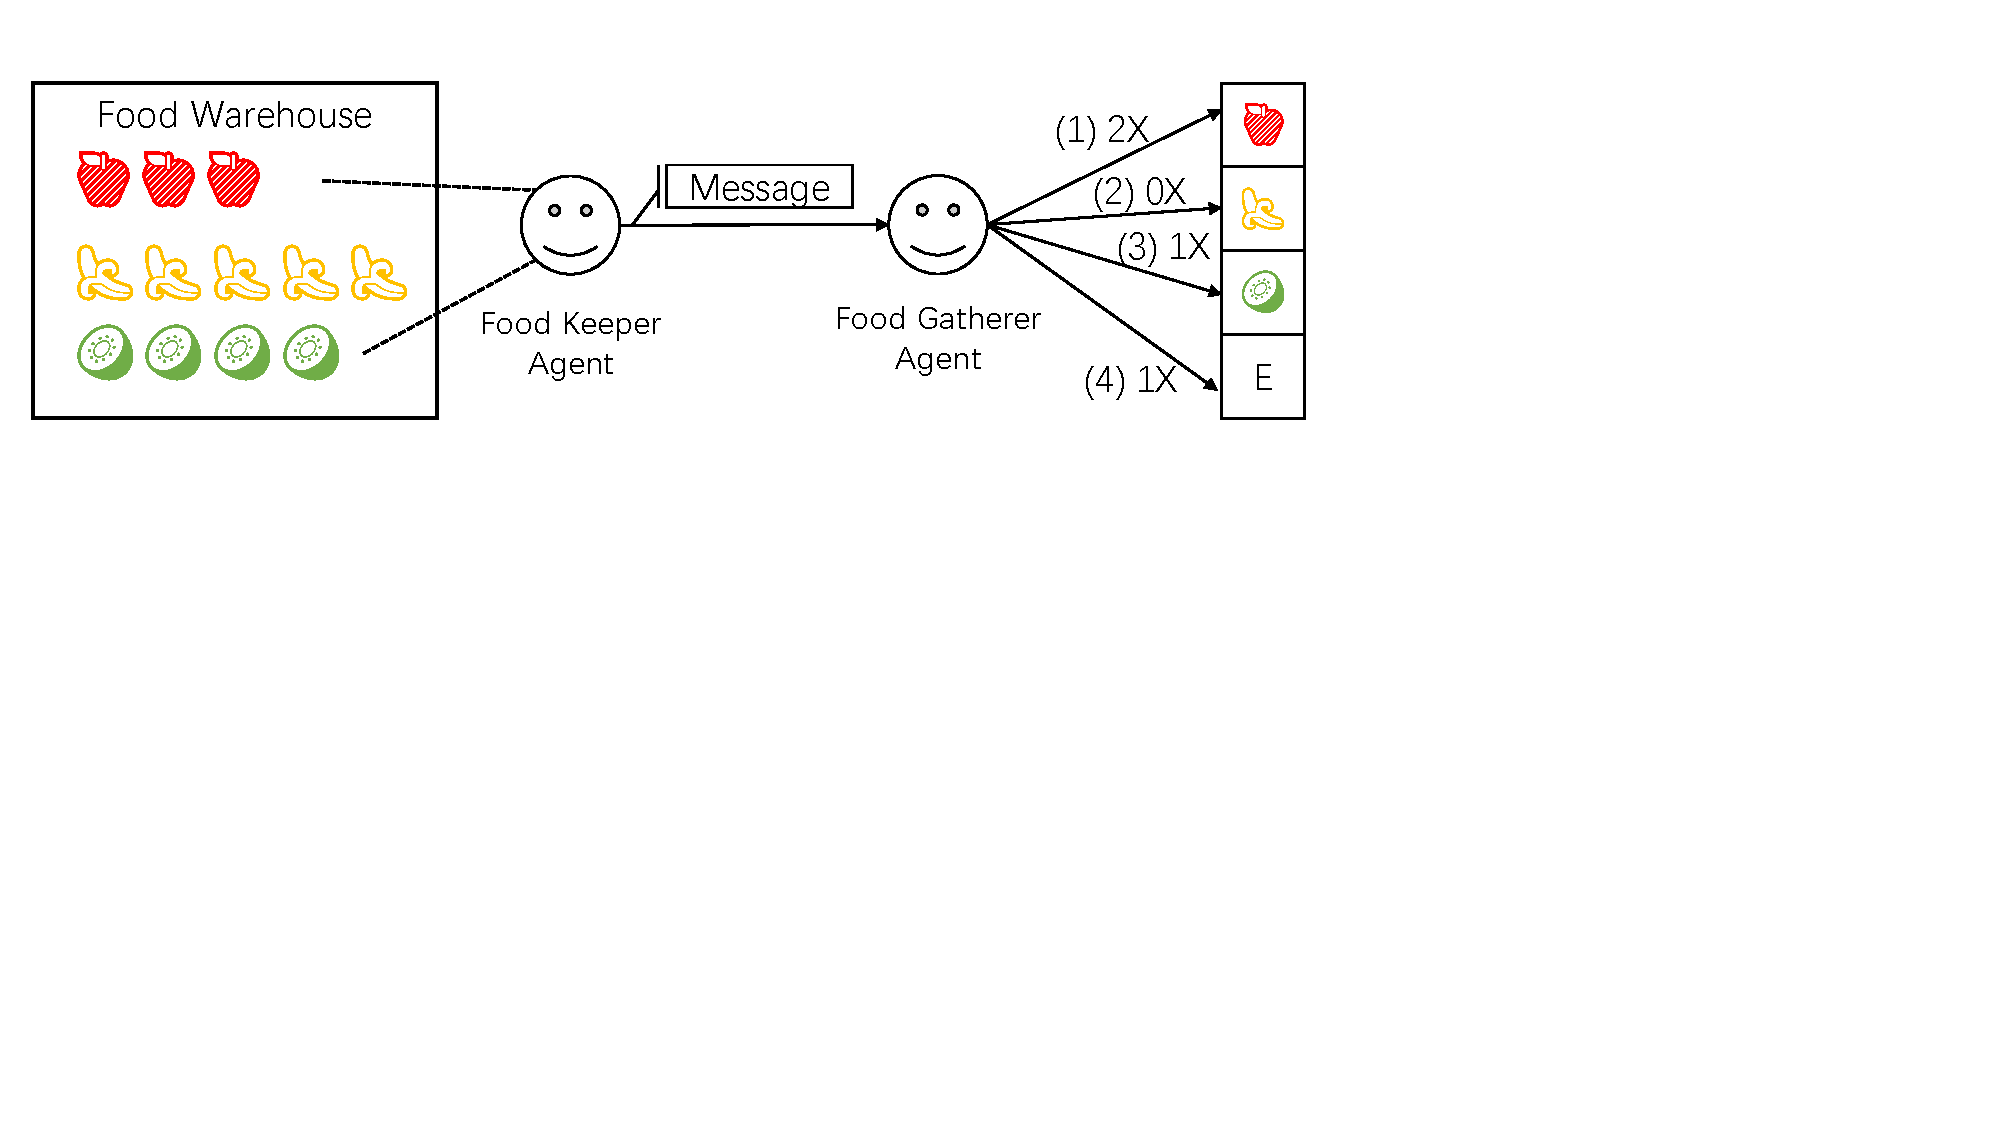
\includegraphics[width=0.6\textwidth]{Diagram.pdf}
  \caption{The diagram of proposed Food-Gathering Bandit Game.}\label{fig:game1}
\end{figure}

In order to better describe our game configuration, we first introduce the following components of FGBG:

\begin{itemize}
  \item Food Warehouse: There is always only 1 specific kind of food in food warehouse whose quantity is initialised randomly from episode to episode. Besides, the quantity is represented as a single integer $n\in \{1, 2, \dots, 5\}$.
  \item Speaking Agent: This is the one that can check status of warehouse and send a message to the other agent. However, its action space is limited such that it can not push the bandit.
  \item Listening Agent: This is the one that first receives message from speaking agent and then can push the bandit according to the message. However, its observation is limited such that it can not observe the status of food warehouse.
  \item 2-armed Bandit: There are only 2 actions that are supported by the 2-armed bandit, i.e. get an apple or end the episode immediately.
  \item Message Channel: Message consist of only one discrete symbols from a vocabulary containing 5 discrete symbols. However, we assume that different reward configuration would lead to different preference of agents and we thus would further illustrate this in the following paragraph.
\end{itemize}

The \textbf{Objective} of FGBG is to fulfill the food warehouse with exactly 5 apples. In the beginning of every episode, speaking agent would first check the status of food warehouse and then send a message to the listening agent. After receiving the message, the listening agent would push the bandits. And, once it pushes the down bandit, the game ends. If the listening agent pushes the down bandit exactly as the numbers needed, i.e. 5 minus numbers of apples already in the food warehouse, both agents would get reward $+100$, otherwise, they would get $-100$. Take the situation in Figure \ref{fig:game1} for example. As there are 3 apples in the food warehouse after initialisation, the desired behaviour of listening agent is to \textit{push the up bandit twice and then push the down bandit} after receiving the message from speaking agent. If so, both agents would get reward $+100$ otherwise $-100$.

With the assumption that all the information need to communicated between two agents is the number of apples in food warehouse, we argue that all the symbols combinations appear as messages should all be combinations of numerals. From a functional perspective, numerals emerged in this game are to describe how many times an action should be executed. Take number $3$ for example, its function is to compress a string consists of 3 same symbols into 1 tokens, i.e.

$$3(apple) = apple \ \ apple\ \ apple$$ .

Ideally, agents could assign every symbol to a specific number. However, it is also possible that meanings of symbols in their communication are not atomic, i.e. they may use successive several symbols to represent a single number like the 8-digits integers in digital computers.

\noindent\textbf{Future Works}

Based on FGBG, we could also alter the components to make the simulation be able to express/reflect more linguistic phenomena related to cardinal numerals. For instance, with a penalisation mechanism on the length of messages, we could further verify the hypotheses about the balance between efficiency and ambiguity of language. Or, by altering the numbers of food types in food warehouse, we could further simulate the emergence of quantifier phrases, e.g. 3 apples and 2 bananas. Without exaggeration, there are still other potentials of our framework.

\label{ssec:3.4garmmar_game}

Unlike cardinal numerals and ordinal numerals, the emergence of numeral grammars are not self-supported but rely on other basic elements in numeral systems. Thus, we propose the following hypotheses that can facilitate the emergence of numeral grammars and, more importantly, can be implied in the proposed simulation framework.

\begin{enumerate}
  \item Dynamic changing objective and dialogue: concepts related to arithmetic operations in numeral grammars become necessary when agents need dialogues to capture the dynamic changing objective during completing tasks. For example, in FGBG, once the speaker agent realised that the status of food warehouse changed, it can directly tell the listener how many more apples are needed, which is a more efficient communication protocol.
  \item Update the existing cardinal numerals: once agents realise the boundness of the existing cardinal numeral systems, they could take n-based positional numeral systems as an update the existing communication protocol (i.e. numeral systems). Assuming that vocabulary could not be enlarged during the simulation, this is the only way for agents to enhance the representation capability of the existing numeral systems.
\end{enumerate}

%\begin{itemize}
%    \item Detail the methodology to be used in pursuit of the research and justify this choice.
%    \item Describe your contributions and novelty and where you
%    will go beyond the state-of-the-art (new methods, new tools,
%    new data, new insights, new proofs,...)
%    \item Describe the programme of work, indicating the research to be undertaken and the milestones that can be used to measure its progress.
%    \item Where suitable define work packages and define the dependences
%    between these work packages. WPs and their dependences should be
%    shown in the Gantt chart in the research plan.
%    \item Explain how the project will be managed.
%    \item State the limitations of your research.
%\end{itemize}

\section{Expected Outcomes}
\label{sec:4outcomes}

As an interdisciplinary project, the expected outcomes of our project are various.

First and foremost, the main contribution of this project is a new computer simulation framework for emergence and evolution of numeral systems as well as other topics in evolutionary linguistics. Our work also fills the gaps between existing works in evolutionary linguistics and hypotheses/thoeries about basic elements of language. Moreover, we provide a more powerful tool to verify the hypotheses and theories in evolutionary linguistics.

Meanwhile, as we follow the reinforcement learning framework, we would also contribute techniques that estimate the gradients of discrete symbols in vocabulary during the end to end multi-agent training procedure.

%Conclude your research proposal by addressing your predicted outcomes. What are you hoping to prove/disprove? Indicate how you envisage your research will contribute to debates and discussions in your particular subject area:
%
%\begin{itemize}
%    \item How will your research make an original contribution to knowledge?
%    \item How might it fill gaps in existing work?
%    \item How might it extend understanding of particular topics?
%\end{itemize}


\section{Research Plan, Milestones and Deliverables}

\definecolor{barblue}{RGB}{153,204,254}
\definecolor{groupblue}{RGB}{51,102,254}
\definecolor{linkred}{RGB}{165,0,33}

\begin{figure}[htbp]
\begin{ganttchart}[
    y unit title=0.4cm,
    y unit chart=0.5cm,
    vgrid,hgrid,
    x unit=1.55mm,
    time slot format=isodate,
    title/.append style={draw=none, fill=barblue},
    title label font=\sffamily\bfseries\color{white},
    title label node/.append style={below=-1.6ex},
    title left shift=.05,
    title right shift=-.05,
    title height=1,
    bar/.append style={draw=none, fill=groupblue},
    bar height=.6,
    bar label font=\normalsize\color{black!50},
    group right shift=0,
    group top shift=.6,
    group height=.3,
    group peaks height=.2,
    bar incomplete/.append style={fill=green}
   ]{2018-06-01}{2018-08-16}
   \gantttitlecalendar{month=name}\\
   \ganttbar[
    progress=100,
    bar progress label font=\small\color{barblue},
    bar progress label node/.append style={right=4pt},
    bar label font=\normalsize\color{barblue},
    name=pp
   ]{Background Reading}{2018-06-01}{2018-06-14} \\
\ganttset{progress label text={}, link/.style={black, -to}}
\ganttgroup{Objective 1}{2018-06-14}{2018-06-30} \\
\ganttbar[progress=4, name=T1A]{Task A}{2018-06-14}{2018-06-21} \\
\ganttlinkedbar[progress=0]{Task B}{2018-06-21}{2018-06-30} \\
\ganttgroup{Objective 2}{2018-07-01}{2018-07-14} \\
\ganttbar[progress=15, name=T2A]{Task A}{2018-07-01}{2018-07-07} \\
\ganttlinkedbar[progress=0]{Task B}{2018-07-07}{2018-07-14} \\
\ganttgroup{Dissertation    }{2018-07-14}{2018-08-16} \\
  \ganttbar[progress=0]{Task A}{2018-07-14}{2018-08-16}
  \ganttset{link/.style={green}}
  \ganttlink[link mid=.4]{pp}{T1A}
  \ganttlink[link mid=.159]{pp}{T2A}
\end{ganttchart}
\caption{Gantt Chart of the activities defined for this project.}
\label{fig:gantt}
\end{figure}

\begin{table}[htbp]
    \begin{center}
        \begin{tabular}{|c|c|l|}
        \hline
        \textbf{Milestone} & \textbf{Week} & \textbf{Description} \\
        \hline
        $M_1$ & 2 & Feasibility study completed \\
        $M_2$ & 5 & First prototype implementation completed \\
        $M_3$ & 7 & Evaluation completed \\
        $M_4$ & 10 & Submission of dissertation \\
        \hline
        \end{tabular}
    \end{center}
    \caption{Milestones defined in this project.}
    \label{fig:milestones}
\end{table}

\begin{table}[htbp]
    \begin{center}
        \begin{tabular}{|c|c|l|}
        \hline
        \textbf{Deliverable} & \textbf{Week} & \textbf{Description} \\
        \hline
        $D_1$ & 6 & Software tool for \dots\\
        $D_2$ & 8 & Evaluation report on \dots\\
        $D_3$ & 10 & Dissertation \\
        \hline
        \end{tabular}
    \end{center}
    \caption{List of deliverables defined in this project.}
    \label{fig:deliverables}
\end{table}

\pagebreak
%                Now build the reference list
\bibliographystyle{unsrt}   % The reference style
%                This is plain and unsorted, so in the order
%                they appear in the document.

{\small
\bibliography{main}       % bib file(s).
}
\end{document}

